\documentclass[12pt,a4paper]{article}
\usepackage[ansinew]{inputenc} 			% Windows
%\usepackage[latin1]{inputenc} 			% Linux og Mac

\usepackage[T1]{fontenc} 
\usepackage[danish]{babel}				% Dansk ordbog
\usepackage{amsmath, amsfonts, amssymb} % Matematiske pakker
\usepackage{graphicx} 					% Grafiksk pakke
\usepackage{float}						% TIL AT BILLEDER BLIVER HVOR DE ER

\usepackage[left	=3cm,
			right	=2cm,
			top		=2.2cm,
			bottom	=2cm
		]{geometry} 					% Sidejustering

%Mellemrum mellem linjerne
\usepackage{setspace}
\setstretch{1.5} %Afstanden

\usepackage{lastpage}

% Links
\usepackage{hyperref}
\hypersetup{ 
	colorlinks	= true, 	% false: boxed links; true: colored links
    urlcolor	= blue,		% color of external links
    linkcolor	= black, 	% color of page numbers
}

% Figur der st�r vilk�rligt
\usepackage{wrapfig}
%\begin{wrapfigure}{r}{0.6\textwidth}
%	\centering
%	\includegraphics[scale=0.25]{...}
%    \vspace{-20pt}
%    \caption{...}
%  \label{fig:...}
%  \vspace{-10pt}
%\end{wrapfigure}

% Sideops�tning
\usepackage{fancyhdr}					% Header-style
\pagestyle{fancy}
\fancyhf{} % slet alt
\fancyfoot[C]{Side \thepage \text{ af} \pageref{LastPage}} % sidetallet yderst
\lhead[]{\leftmark} % lige side, kapitel titel
\headheight = 35pt
\textheight = 680pt
\footskip 	= 40pt
\rhead{
\begin{picture}(0,0)
\put(-120,0){ \includegraphics[scale=0.2]{au-ingenioerhoejskolen_da.jpg}}
\end{picture}}
\renewcommand{\headrulewidth}{0.4pt}
\renewcommand{\footrulewidth}{0.4pt}

\usepackage{enumerate}

\usepackage{subfiles}

%----------------------------------------------------------
% F�lgende er til tabeller
%----------------------------------------------------------
\usepackage{booktabs, cellspace} 		
\addtolength\cellspacetoplimit{10pt}
\addtolength\cellspacebottomlimit{10pt}

%----------------------------------------------------------
% F�lgende er til koder.
% Inds�ttes mellem \begin{lstlisting} og \end{lstlisting}
%----------------------------------------------------------
\usepackage{listings}
\usepackage{color}
\usepackage{textcomp}
\definecolor{listinggray}{gray}{0.9}
\definecolor{lbcolor}{rgb}{0.9,0.9,0.9}
\lstset{
	language		= [Sharp]C,
	keywordstyle	= \bfseries\ttfamily\color[rgb]{0,0,1},
	identifierstyle	= \ttfamily,
	commentstyle	= \color[rgb]{0.133,0.545,0.133},
	stringstyle		= \ttfamily\color[rgb]{0.627,0.126,0.941},
	showstringspaces= false,
	basicstyle		= \small,
	numberstyle		= \footnotesize,
	numbers			= left, % Tal? Udkommenter hvis ikke
	stepnumber		= 1,
	numbersep		= 5pt,
	tabsize			= 2,
	breaklines		= true,
	prebreak 		= \raisebox{0ex}[0ex][0ex]{\ensuremath{\hookleftarrow}},
	breakatwhitespace= false,
	aboveskip		= {1.5\baselineskip},
  	columns			= fixed,
  	upquote			= true,
  	extendedchars	= true,
	lineskip		= 1.5pt,
    xleftmargin		= 17pt,
	framexleftmargin= 17pt,
	framexrightmargin	= 5pt,
	framexbottommargin	= 4pt,
% frame=single,
 	backgroundcolor=\color{lbcolor},
}
\renewcommand*{\lstlistingname}{Kodeudsnit}

\usepackage{caption}
\DeclareCaptionFont{white}{\color{white}}
\DeclareCaptionFormat{listing}{\colorbox[cmyk]{0.43, 0.35, 0.35,0.01}{\parbox{\textwidth}{\hspace{15pt}#1#2#3}}}
\captionsetup[lstlisting]{format=listing,labelfont=white,textfont=white, singlelinecheck=false, margin=0pt, font={bf,footnotesize}}


%----------------------------------------------------------
% F�lgende er tabel over Use Cases - Akt�rer - Forventet 
% 	resultat og checkbox
% Inds�ttes med \begin{testcase} og \end{testcase}
%----------------------------------------------------------
%\usepackage{enumitem,calc}

\newenvironment{testcase}[1]
{
\begin{tabular}{| p{1.2cm} | p{6cm} | p{5.5cm} | l|}\hline
\textbf{TRIN} & \textbf{Aktion / Input} & \textbf{Forventet resultat} & \textbf{CHK} \\
\hline
}
{&\\\hline
\end{tabular}
\\\\}
\newcommand\punkt{&\\\hline} 
\newcommand\Aktion{&}
\newcommand\Forventet{&}

%Grader tegn
\newcommand{\degree}{\ensuremath{^\circ}}

%Bilag kommando
\providecommand{\Bilag}
{ 	\cleardoublepage
	\appendix % Sletter alle kapitelnumre og starter forfra
	\renewcommand{\appendixname}{Bilag} % Fort�ller navnet skal v�re "Bilag"
	\part*{Bilag}
	\addcontentsline{toc}{part}{Bilag}
	\renewcommand{\thesection}{\Roman{section}}
}

% Paragraph instillinger
\renewcommand\paragraph{\@startsection{paragraph}{4}{\z@}%
  {-3.25ex\@plus -1ex \@minus -.2ex}%
  {1.5ex \@plus .2ex}%
  {\normalfont\normalsize\bfseries}}	% Alle indstillinger for dokumentet

%***************************************************
% Det afsnit du arbejder p� skal skrives her
% Inklud�r flere afsnit med komma
% Udkommenter alt du ikke skal bruge med '%'
%
\includeonly{
	Andre_afsnit/Forside,
	Indledning/FormAl,
	Generel_Beskrivelse/Systembeskrivelse,
	Generel_Beskrivelse/Systemets_funktioner,
	Use_Cases/Funktionelle_krav, %Her i ligger Use_Case1
	Use_Cases/Use_Case2,
	Use_Cases/Use_Case3,
	Use_Cases/Use_Case4,
	Use_Cases/Use_Case5,
	Use_Cases/Use_Case6,
	Use_Cases/Use_Case7,
	Use_Cases/Use_Case8,
	Eksterne_grEnseflader/Ekstern,
	Andre_afsnit/Kvalitetsfaktorer,
	Andre_afsnit/Designkrav,
	%Andre_afsnit/Ovrigekrav,
	%Andre_afsnit/Delleveringer,
}
%***************************************************

\begin{document}

%---------------------------------------------------
%Herunder skal alle kapitlerne st�.
%
%Hvis der tilf�jes et afsnit, skal det ogs� inkluderes 
%under afsnittet ovenover - adskildt med et komma.
%Tilf�j dit afsnit herunder og udkommenter over over.
%---------------------------------------------------

\newcommand{\HRule}{\rule{\linewidth}{0.8mm}}
\author{TrackABus\\\\Bachelorgr. 13038}
\title{Kravspecifikation}
\date{}

\begin{titlepage}

\begin{center}


% Upper part of the page]    

\textsc{\LARGE TrackABus}\\[1.5cm]

\textsc{\Large Bachelorprojekt}\\[0.5cm]


% Title
\HRule \\[0.4cm]

{ \huge \bfseries Kravspecifikation}\\[0.4cm]
{ \huge \bfseries for}\\[0.4cm] 
{ \huge \bfseries TrackABus}\\[0.4cm]

\HRule \\[1.5cm]

% Author and supervisor
\begin{minipage}{0.4\textwidth}
\begin{flushleft} \large
\emph{Author:}\\
Bachelorgruppe 13038
\end{flushleft}
\end{minipage}
\begin{minipage}{0.4\textwidth}
\begin{flushright} \large
\emph{Supervisor:} \\
Michael Alr�e
\end{flushright}
\end{minipage}

\vfill

% Bottom of the page
{\large \today}

\end{center}

\end{titlepage}

\newpage
\section*{Versionshistorie}


    \begin{tabular}{ | l | l | l | p{10cm} |}
    \hline
    Ver. & Dato & Initialer & Beskrivelse \\ \hline
    0.3 & 06.03.2012 & Gruppe 5 & Skabelon til kravspecifikationen udf�rdiget. \\ \hline
    1.0 & 20.03.2012 & Gruppe 5 & Krav udf�rdiget, mange stadig som brief og casual Use Cases. \\ \hline
    2.0 & 15.04.2012 & Gruppe 5 & Alle Use Cases udf�rdiget som fully dressed. \\ \hline
    3.0 & 17.05.2012 & Gruppe 5 & Dokumentet udf�rdiget til endelig aflevering. \\ \hline
    \end{tabular}

\section*{Godkendelsesformular}
    
    \begin{tabular}{ | l | p{12.4cm} |}
    \hline
    Forfattere 			& Projekt gruppe 5 \\ \hline
    Godkendes af 		& Kunde: Poul Ejnar Rovsing \\& 
    Leverand�r Repr�sentant: Lars Anker Christensen \\ \hline
    Projektnummer 		& 4. Semester projekt \\ \hline
    Dokument-id 		& SBS\_Kravspecifikation \\ \hline
    Antal sider & 31 \\ \hline
    kunde & Poul Ejnar Rovsing \\ \hline
    \end{tabular}  
\\\\
\textbf{Ved underskrivelse af dette dokument accepteres det af begge parter, som v�rende kravene til udviklingen af det �nskede system.}
\\
\\
\textbf{Sted og dato:} \line(1,0){105}
\vspace{1.5cm}
\newpage

\vspace*{1cm}
\begin{tabular}{llp{3cm}ll}
\cline{5-5}
&&&09421 & Lasse Lindsted S�rensen		\\\\\\\cline{5-5}
&&&10063 & Lasse Hansen					\\\\\\\cline{5-5}
&&&10648 & Lars Anker Christensen		\\\\\\\cline{5-5}
&&&10719 & Michael Bojsen-Hansen		\\\\\\\cline{5-5}
&&&10750 & Kasper Vinther Andersen		\\\\\\\cline{5-5}
&&&10770 & Christian Smidt-Jensen		\\\\\\\cline{5-5}
&&&10832 & Christoffer Lousdahl Werge	\\\\\\\cline{5-5}
\cline{1-2} PER & Poul Ejnar Rovsing &&10893 & Rasmus B�kgaard
\end{tabular}

\newpage
\tableofcontents



%1. INDLEDNING
\section{Indledning}

\subsection{Form�l}
Dette dokument har til form�l at opstille de krav, der skal v�re opfyldt, n�r projektet er f�rdiggjort. Dokumentet er blevet udformet af projektgruppe 5, der skal udf�rdige produktet, og sikre at kravene i dette dokument er opfyldt. 
\\
De forskellige krav til produktet, er blevet udformet i samarbejde med kunden, som i dette tilf�lde er projektgruppens eget firma. Derved er det blevet sikret, at misforst�elser bliver undg�et. B�de kunden og projektgruppen har underskrevet dokumentet, som tegn p� deres indforst�else med kravene. 
\\
Der er taget forbehold for, at ny viden vil blive indsamlet under produktudviklingen, og derfor ser projektgruppen sig berettiget til at g� tilbage og tilpasse Kravspecifikationen, s� dokumentet forbliver opdateret. Der vil naturligvis \underline{KUN} ske �ndringer i dokumentet, hvis kunden kan acceptere �ndringerne og er indforst�et med f�lgerne af disse.

\subsection{Referencer}
F�lgende dokumenter refereres der til i kravspecifikationen
\begin{itemize}
	\item SBS\_Ide-funktioner.
	\item SBS\_HardwareSpec.
	\item Scorbot-ER 4u, Users Manual -- 100343b ER 4u.
\end{itemize}\
Udover disse dokumenter, er der lavet en accepttest specifikation, der st�r for at verificere at kravene er opfyldt.

\subsection{L�sevejledning}
F�rst skal det n�vnes at det er valgt at kalde systemet for Silver Bullet Sort (SBS), s� l�ser ikke er i tvivl n�r dette navn fremg�r at kravspecifikationen. Derudover ses herunder en kort beskrivelse af de forskellige afsnit:
\\
\begin{itemize}
\item General Beskrivelse\\
I starten af dokumentet beskrives og illustreres systemet i sin helhed, samt et overblik over systemet funktioner gives.\\

\item Funktionelle krav\\
Her er alle Use Cases beskrevet fully dressed.\\

\item Eksterne Gr�nseflader\\
Her ses en skitse over hvordan brugergr�nsefladen vil komme til at se ud. Derudover er Hardwarens gr�nseflader beskrevet. Hardwarens gr�nseflader beskrives dog kun overfladisk 

\item Kvalitetsfaktorer og Designkrav\\
Her er beskrevet den kvalitet og den ydelse kunden kan forvente. Derudover kan her ogs� l�ses, hvilke krav der stilles til designer, i forbindelse med implementering\\
 
\item Dellevering\\
Her er beskrevet, hvilke leverancer kunden kan forvente

\end{itemize}


%2. Generel Beskrivelse
\section{Generel beskrivelse}

\subsection{Systembeskrivelse}

\begin{itemize}

\item Brugersystem \\
Brugersystemet st�r til ansvar for, at brugeren f�r en intuitiv indgang til systemet. Dette system d�kker hele brugeroplevelsen, herunder at kunne v�lge en busrute og se denne p� kortet. Brugersystemet d�kker intet administrativt, og brugeren skal ikke have nogen specielle evner for at bruge denne del af systemet.

\item Administrations system  \\ 
Administrations systemet st�r til ansvar for, at administratoren kan �ndre persisteret data nemt, uden at skulle tilg� databasen direkte. Dette systeme d�kker over en r�kke v�rkt�jer som kan manipulere data for busser og deres ruter. Systemet har ingen p�virkning p� brugersystemet, ud over de �ndringer der sker p� persisteret data.

\item Positionsdata \\
Positionsdata, er infomrationen om bussens placering. Position persisteres direkte, uden om administrations systemet og brugersystemet. Denne del kan simuleres uden tab af funktionalitet.

\item Distribueret persisteret data \\
Persisteret data er kerneelementet i dette projekt. Persisteret data er to-delt og best�r i den globale persisterede data og lokalt persisteret data. Globalt persisteret data vil best� af alt den information brugersystemet og administrations systemet har til f�lles, hvor et eksempel kunne v�re positionsdata. Lokalt persisteret data vil best� af den information brugeren har valgt at gemme lokalt fra brugersystemet, dette vil prim�rt best� af favoriserede busruter. 

\item Lokalt Distribueret data
\end{itemize}

\begin{figure}[u]
\centering
\includegraphics[scale=0.7]{Domainmodel_Billede.jpg}
\caption{Dom�nemodel}
\label{domainmodel}
\end{figure} 

p� figur \ref{domainmodel} gives der et overblik over systemet, hvor enhederne ses i sammenh�ng. De forskellige enheder er beskrevet kort i ovenst�ende afsnit, \emph{2.1 Systembeskrivelse}. Diagramet er lavet med online-v�rk�jet creately.com.

%\subsubsection{Akt�r kontekst-diagram}

\begin{figure}[h]
\centering
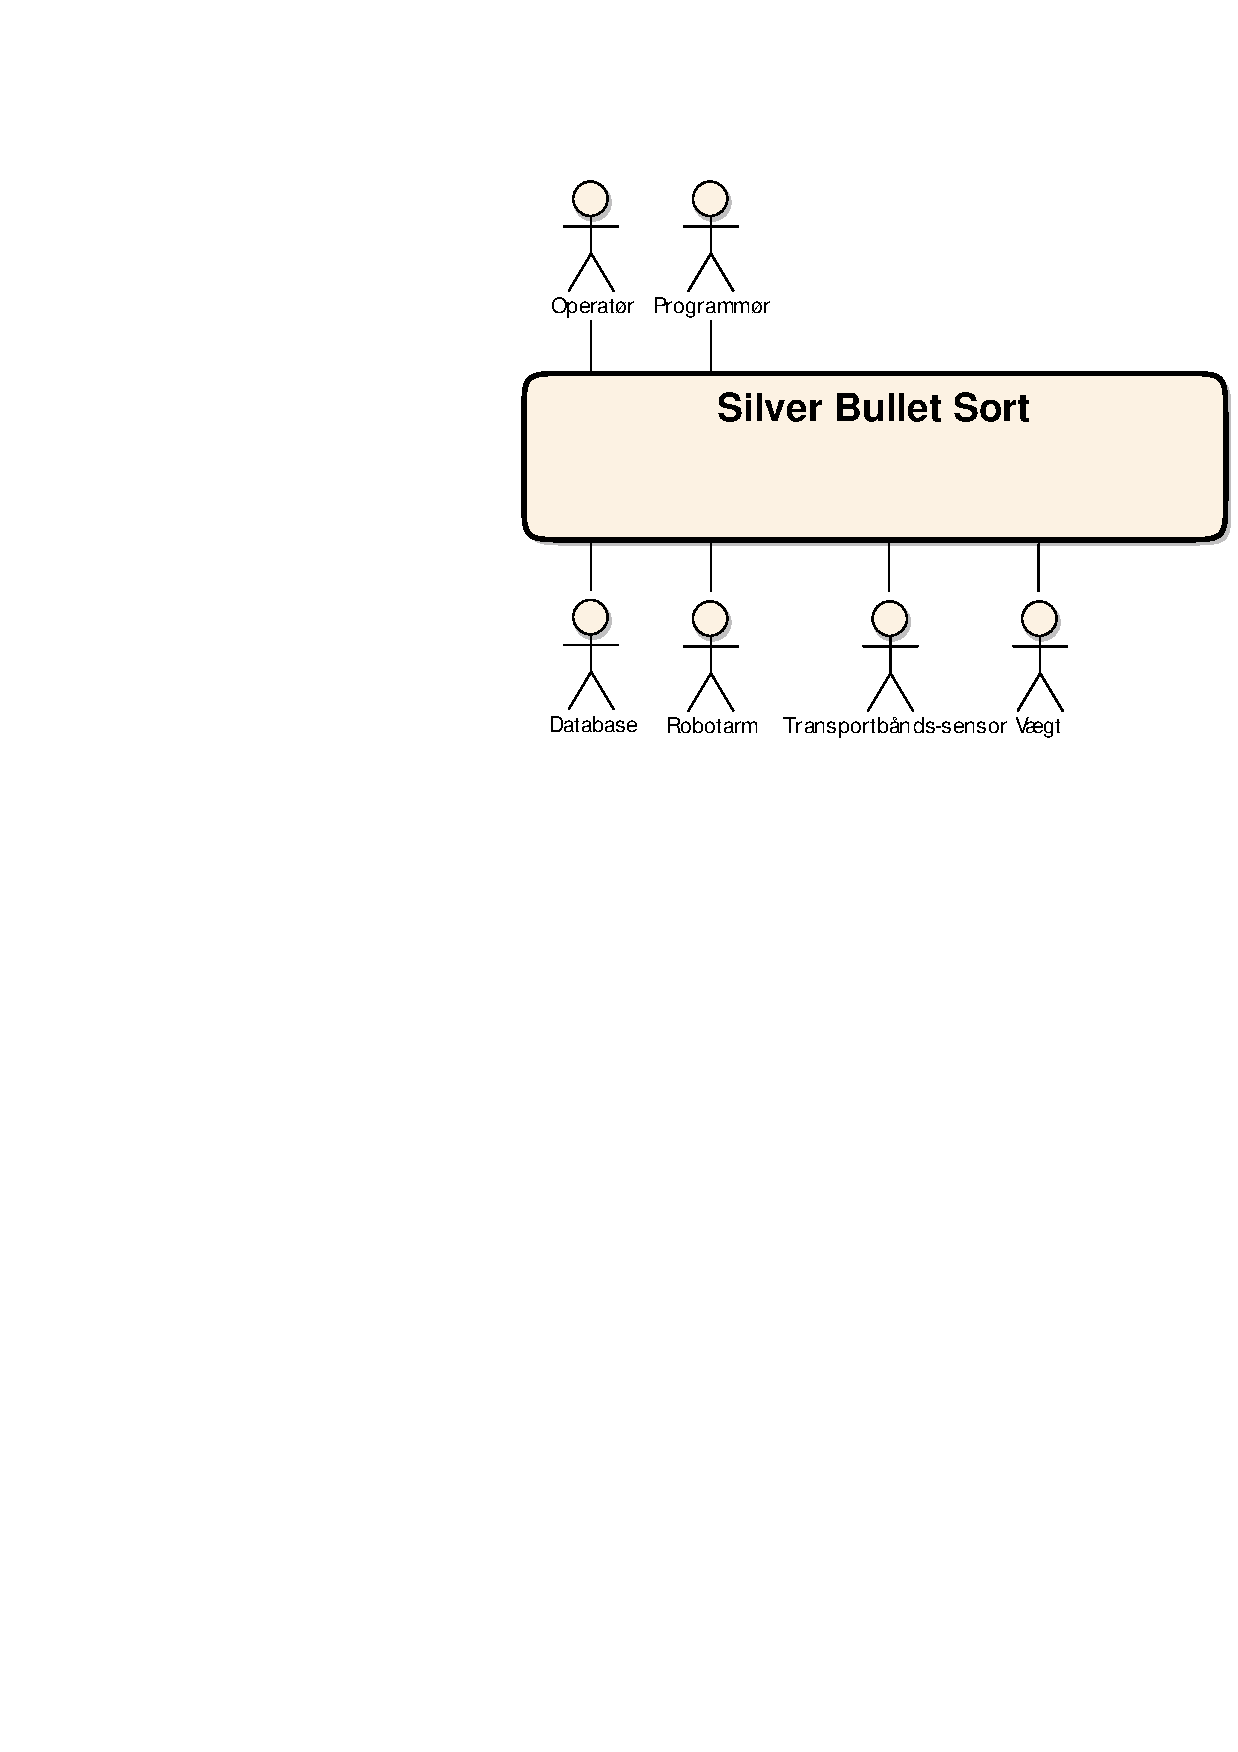
\includegraphics[scale=0.5]{Andet/AktOr-kontekst.jpg}
\caption{Akt�r kontekst-diagram}
\end{figure}

Ovenst�ende figur viser hvilke akt�rer, der interagerer med sorteringssystemet. Videre beskrivelse af disse akt�rer, findes i f�lgende afsnit \emph{2.1.3 Akt�rbeskrivelser}  
\newpage

%\subsubsection{Akt�r beskrivelse}

\underline{\textbf{Prim�re akt�rer:}}\\
\begin{tabular}{lp{10 cm}}

\textbf{Akt�r navn} 				& Operat�r\\
\textbf{Beskrivelse} 				& Denne akt�r starter og stopper systemet. M�let for akt�ren er at f� sorteret klodser, alt efter deres materialetype. \\
\textbf{Antal samtidige akt�rer}	& 1 \\
\\\\
\textbf{Akt�r navn}					&  Programm�r. \\ 
\textbf{Beskrivelse} 				&  Denne akt�rs opgave er at lave brugerdefinerede programmer til systemet.\\ 
\textbf{Antal samtidige akt�rer} 	&  1
\end{tabular}
\\\\
\\\\
\underline{\textbf{Sekund�re akt�rer}}
\\
\begin{tabular}{lp{10 cm}}

\textbf{Akt�r navn} 				& V�gt\\
\textbf{Beskrivelse} 				& Denne akt�r vejer et objekt, s� systemet kan bestemme dets materialetype.  \\
\textbf{Antal samtidige akt�rer}	& 1 \\
\\\\
\textbf{Akt�r navn}					& Transportb�ndssensor \\
\textbf{Beskrivelse}				& Denne akt�r registrerer, hvorn�r et objekt er klar til at blive samlet op af robotten.  \\
\textbf{Antal samtidige akt�rer}	& 1 \\
\\\\
\textbf{Akt�r navn} 				&  Robotarm.\\ 
\textbf{Beskrivelse} 				&  Denne akt�rs opgave er at flytte og m�le forskellige typer klodser.\\ 
\textbf{Antal samtidige akt�rer} 	&  1 \\ 
\\\\
\textbf{Akt�r navn} 				&  Database. \\ 
\textbf{Beskrivelse} 				&  Databasen indeholder logfiler for systemets data for de enkelte klodser, samt informationer om robotten og systemets status. Ligeledes indeholder databasen programmerne, som programm�ren har lavet.\\ 
\textbf{Antal samtidige akt�rer} 	&  1
\end{tabular} 


\subsection{Systemets funktioner}
I det f�lgende punkt er systemets funktioner beskrevet ved Use Case-teknikken. P� figur \ref{usecasediagram} gives der et overblik over systemets funktioner

\subsubsection{Use Case diagram}

\begin{figure}[h]
\centering
\includegraphics[scale=0.6]{Use_Cases/Diagrammer/Use_Case_Diagram.jpg} 
\caption{Use Case diagram}
\end{figure}

Hovedfunktionen i systemet er, at lade en bruger finde ud, hvor en given bus befinder sig p� et rute, ud fra et valgt stoppested. Brugeren vil v�lge en rute, hvorefter han vil kunne se alle busser p� den valgte rute. Herefter vil han kunne v�lge et stoppested, og herefter vil kun den n�rmeste (og muligvis n�stn�rmeste, se Use Case 3, undtagelse 5) vises p� kortet. Udover dette vil en estimeret tid, for ankomst af den n�rmeste bus til stoppestedet, vises.
\\ 
En administrator kan �ndre ruteplaner, busser og busnumre i et seperat system.\\\\
De forskellige Use Cases er detaljeret beskrevet senere i dokumentet, i afsnittet \textit{3 Funktionelle krav - Use Cases}
\subsection{Systemets begr�nsninger}
I produktopl�gget er et kamera beskrevet. I det endelige produkt er dette erstattet af en optisk sensor, som indg�r i styringen af transportb�ndet. Dette er foretaget efter aftale med kunde.\\
Den manuelle pendant er desuden fjernet, og i stedet kan robotten programmeres via et user interface p� en PC.

\subsection{Brugerprofil}
\begin{itemize}

\item Brugeren \\
Brugeren er en prim�r akt�r af systemet. Det er ikke essentielt at denne person har nogen forst�else for, hvad der foreg�r bag systemet. Det eneste krav der stilles til brugeren er, at personen skal tilg� systemet fra en android platform.
\item Administrator \\
Administratoren er en prim�r akt�r af systmet. Det er ikke essentielt at denne person har forst�else for, hvordan en database virker. Det er dog vigtigt at personen er tr�net i at bruge denne del af systemet, og har en forst�else for, hvad de �ndringerne der foretages, g�r. Da administratoren bliver pr�senteret for et r�kke v�rkt�j, skal personen ikke n�dvendigvis have specielle kompetencer.

\end{itemize}


\subsection{Krav til udviklingsforl�bet}
Selvom der ikke blev vedlagt mange obligatoriske krav til dette projekt, er der i gruppen blevet fastlagt nogle udviklingsm�ssige rammer, som vil blive fulgt:

\subsubsection{Obligatoriske udviklingsv�rkt�jer}
Programmeringssproget skal i dette projekt v�re C\#, hvor der skal g�res brug af WPF til det grafiske interface samt .NET 4.0 frameworket. Til persistente data skal der g�res brug af SQL databaser, herunder logning og lagering af data fra klodserne. Undervejs i projektet udarbejdes to store dokumenter, en processrapport og et designdokument. \\

\subsubsection{Gruppedefinerede udviklingsv�rkt�jer}
Til selve udviklingen er der blevet valgt at f�lge v�sentlige principper fra Scrum frameworket. Der blev gjort brug af dette i tredje semesterprojektet, hvor det blev set som ganske brugbart. Herunder blev der ogs� gjort brug af nogle af Extreme Programming-principperne. \\ 




\subsection{Foruds�tninger}
Det forventes at der kan skabes en l�bende kommunikation med kunden (Michael Alr�e, ma@iha.dk). Hertil vil der l�bende blive holdt m�der, hvor �ndringer diskuteres.


\subsection{Systemets begr�nsninger}
I produktopl�gget er et kamera beskrevet. I det endelige produkt er dette erstattet af en optisk sensor, som indg�r i styringen af transportb�ndet. Dette er foretaget efter aftale med kunde.\\
Den manuelle pendant er desuden fjernet, og i stedet kan robotten programmeres via et user interface p� en PC.

\subsection{Brugerprofil}
\begin{itemize}

\item Brugeren \\
Brugeren er en prim�r akt�r af systemet. Det er ikke essentielt at denne person har nogen forst�else for, hvad der foreg�r bag systemet. Det eneste krav der stilles til brugeren er, at personen skal tilg� systemet fra en android platform.
\item Administrator \\
Administratoren er en prim�r akt�r af systmet. Det er ikke essentielt at denne person har forst�else for, hvordan en database virker. Det er dog vigtigt at personen er tr�net i at bruge denne del af systemet, og har en forst�else for, hvad de �ndringerne der foretages, g�r. Da administratoren bliver pr�senteret for et r�kke v�rkt�j, skal personen ikke n�dvendigvis have specielle kompetencer.

\end{itemize}


\subsection{Krav til udviklingsforl�bet}
Selvom der ikke blev vedlagt mange obligatoriske krav til dette projekt, er der i gruppen blevet fastlagt nogle udviklingsm�ssige rammer, som vil blive fulgt:

\subsubsection{Obligatoriske udviklingsv�rkt�jer}
Programmeringssproget skal i dette projekt v�re C\#, hvor der skal g�res brug af WPF til det grafiske interface samt .NET 4.0 frameworket. Til persistente data skal der g�res brug af SQL databaser, herunder logning og lagering af data fra klodserne. Undervejs i projektet udarbejdes to store dokumenter, en processrapport og et designdokument. \\

\subsubsection{Gruppedefinerede udviklingsv�rkt�jer}
Til selve udviklingen er der blevet valgt at f�lge v�sentlige principper fra Scrum frameworket. Der blev gjort brug af dette i tredje semesterprojektet, hvor det blev set som ganske brugbart. Herunder blev der ogs� gjort brug af nogle af Extreme Programming-principperne. \\ 




\subsection{Foruds�tninger}
Det forventes at der kan skabes en l�bende kommunikation med kunden (Michael Alr�e, ma@iha.dk). Hertil vil der l�bende blive holdt m�der, hvor �ndringer diskuteres.


%3. Use Cases
\section{Funktionelle krav - Use Cases}
\subsection{Use Case 1: Vis liste af Busruter}
\textbf{M�l:}
\\
M�let med denne Use Case er at f� vist en liste af alle persisterede busruter. 
\\
\\
\textbf{Initiering:}
\\
Brugeren tilkendegiver over for systemet, at han �nsker at f� vist en liste af alle persisterede busruter. 
\\
\\
\textbf{Akt�rer og interessenter:}
\\
Prim�re akt�rer:
\begin{itemize}
\item Bruger.
\end{itemize}
\textbf{Antal samtidige forekomster:}
\\
En samtidig forekomst.
\\
\\
\textbf{Ikke funktionelle krav:}
\begin{enumerate}
\item Mere kommer senere
\end{enumerate}
\textbf{Startbetingelser:}
\\
Programmet er startet op, og brugeren st�r ved startsk�rmen.
\\
\\
\textbf{Slutresultat ved succes:}
\\
Brugeren f�r vist en liste over alle persisterede busruter. 
\\
\\
\textbf{Slutresultat ved undtagelser:}
\\
Klodsen er ikke blevet lagt i et rum, hvori materialetypen ikke tilh�rer.
\\
Brugeren bliver pr�senteret for en fejlmeddelelse, der informerer om, at det ikke var muligt at tilg� persisteret data. Desuden f�r brugeren en kort beskrivelse af, hvad der gik galt.
Hvis systemet g�r i dvale, vil listen blive indl�st f�rdig i baggrunden. 
\\
\\
\textbf{Normalforl�b:}

\begin{enumerate}
\item Brugeren tilkendegiver over for systemet, at han �nsker at blive vist listen af busruter.
\item Systemet tilg�r persisteret data, og henter listen af busruter.
\item Systemet pr�senterer brugeren overfor listen af busruter.
\end{enumerate}
\textbf{Undtagelser:}
\begin{enumerate}[\text{Undtagelse} 1:] 
\item Persisteret data kan ikke tilg�s.

	\begin{enumerate}[A]
	\item Systemet viser en fejlmeddelelse til brugeren, der beskriver, at det ikke er muligt at indl�se listen af busruter.
	\item Systemet returnerer til startsk�rmen.
	\end{enumerate}
\end{enumerate}

\begin{enumerate}[\text{Undtagelse} 2:] 
\item Brugeren annullerer indl�sningen. 
	\begin{enumerate}[A]
	\item Systemet annullerer indl�sningen af data.
	\item Systemet returnerer til startsk�rmen.
	\end{enumerate}
\end{enumerate}

\begin{enumerate}[\text{Undtagelse} 3:] 
\item Systemet g�r i dvale, under indl�sningen. 
	\begin{enumerate}[A]
	\item Systemet indl�ser listen af busruter f�rdig i baggrunden.
	\item Hvis brugeren tilg�r systemet igen og listen er hentet f�rdig, vil brugeren blive pr�senteret for listen. Hvis listen endnu ikke er blevet indl�st, vil dette ske i forgrunden.
	\end{enumerate}
\end{enumerate}
\subsection{Use Case 2: F� placering af alle busser og stoppesteder p� valgt rute}
\textbf{M�l:}
\\
M�let med denne Use Case er at f� vist alle busser samt busstoppesteder, for en valgt rute, p� kortet. Busstoppesteder og busser vil v�re tydeligt markeret.
\\
\\
\textbf{Initiering:}
\\
Brugeren tilkendegiver over for systemet, hvilken busrute han �nsker f� vist p� kortet. Alternativt kan brugeren v�lge en favoritrute, givet at favoritrute er tilf�jet, igennem Use Case 4. Brugeren vil da f� vist en busrute, samt hvor p� ruten, busserne og busstoppestederne befinder sig.
\\
\\
\textbf{Akt�rer og interessenter:}
\\
Prim�re akt�rer:
\begin{itemize}
\item Brugeren
\end{itemize}
\textbf{Antal samtidige forekomster:}
\\
En samtidig forekomst.
\\
\\
\textbf{Ikke funktionelle krav:}
\begin{itemize}
\item Kommer senere.
\end{itemize}
\textbf{Startbetingelser:}
\\
Initialisering kr�ver, at en af normalforl�bene for f�lgende Use Cases er fuldendt:
\begin{itemize}
\item Use Case 4 - Tilf�j/Fjern busnummer til listen af favoritter.
\begin{itemize}
\item Hvis en favoritrute i forvejen er tilf�jet, kan Use Case 2 startes fra hovedsk�rmen.
\end{itemize}
\item Use Case 1 - Vis liste af busruter
\begin{itemize}
\item Alle busruter pr�senteres som en liste, efter fuldendt normalforl�b for Use Case 1.
\end{itemize}
\end{itemize}
\textbf{Slutresultat ved succes:}
\\
Brugeren vil blive pr�senteret for et kort, hvorp� busruten er tegnet ind, med tydeligt markerede busstoppesteder. Hvis GPSen i telefonen er sl�et til, vil kortet zoome ind til brugerens position. Hvis GPSen ikke er sl�et til, vil brugeren blive pr�senteret for et kort, zoomet ud til at se hele ruten. P� ruten vil alle k�rende busser, deres retning samt busstoppestederne blive tydeligt vist.
\\
\\
\textbf{Slutresultat ved undtagelser:}
\\
Brugeren vil blive pr�senteret for en fejlmeddelelse, hvori brugeren f�r besked p�, at persisteret data ikke kunne tilg�s. Hvis undtagelsen sker ved, at systemet g�r i dvale, vil ingen data blive indl�st.
\\
\\
\textbf{Normalforl�b:}

\begin{enumerate}[1.]
\item To samtidige operationer:
\begin{enumerate}[A]
\item Kortet vil �bnes og blive vist.
\item Busruten og stoppesteder vil blive hentet fra persisteret data.
\end{enumerate}
\item N�r Busruten og stoppestederne er hentet vil disse indtegnes p� kortet.
\begin{enumerate}[A]
\item Hvis GPS er sl�et til, vil kortet zoome til brugerens position.
\item Hvis GPS ikke er sl�et til, vil kortet zoome s� hele ruten vil blive pr�senteret.
\end{enumerate}
\item Busserne p� den valgte rute, vil f� hentet deres position.
\item Busserne p� den valgte rute, vil f� deres position tegnet ind, tydeligt markeret med den k�rende retning.
\item Efter et tidsinterval, vil alle busser p� ruten, f� deres positionen hentet igen.
\item N�r alle bussernes positioner er hente, vil deres position p� kortet opdateres.
\\\\\\
\end{enumerate}
\textbf{Undtagelser:}
\begin{enumerate}[\text{Undtagelse} 1:] 
\item Hentningen af data annulleres. 
	\begin{enumerate}[A]
	\item Systemet stopper med at hente bussernes positions data.
	\item Der returneres til listen over busruter.
	\end{enumerate}
\end{enumerate}
\begin{enumerate}[\text{Undtagelse} 2:] 
\item Systemet g�r i dvale, under hentning af data. 
	\begin{enumerate}[A]
	\item Hentningen g�res f�rdige, og v�rdier opdateres.
	\item Systemet g�r i dvale. Bussernes position vil ikke l�ngere holdes opdateret.
	\end{enumerate}
\end{enumerate}
\begin{enumerate}[\text{Undtagelse} 3:] 
\item Positions data for busserne kan ikke tilg�s. 
	\begin{enumerate}[A]
	\item Systemet viser en fejlmeddelelse til brugeren, der beskriver, at det ikke er muligt at indl�se bussernes position.
	\item Kortet vil blive vist, hvor busserne er p� deres senest hentede position. Bussernes position opdateres ikke l�ngere.
	\end{enumerate}
\end{enumerate}
\begin{enumerate}[\text{Undtagelse} 4:] 
\item Positions data for busserne kan igen tilg�s. 
	\begin{enumerate}[A]
	\item Systemet forts�tter i normalforl�bet. Bussernes position holdes igen opdateret.
	\end{enumerate}
\end{enumerate}

\subsection{Use Case 3: Rediger materialetype}
\textbf{M�l:}
\\
M�let med denne Use Case er, at tilf�je, �ndre eller fjerne en materialetype.
\\
\\
\textbf{Initiering:}
\\
Use Casen initieres, n�r programm�ren tilkendegiver overfor systemet, at han vil redigere materialetyper.
\\
\\
\textbf{Akt�rer og interessenter:}
\\
Prim�re akt�rer:
	\begin{itemize}
	\item Programm�r.
	\end{itemize}
Sekund�re akt�rer:
	\begin{itemize}
	\item Databasen.
	\end{itemize}
\textbf{Antal samtidige forekomster:}
\\
En samtidig forekomst.
\\\\
\textbf{Ikke funktionelle krav:}
\begin{itemize}
\item Densiteten skal v�re st�rre end 0 $\dfrac{g}{cm^{3}}$ og mindre end 23 $\dfrac{g}{cm^{3}}$.
\end{itemize}
\textbf{Referencer:}
\\
Ingen.
\\\\
\textbf{Startbetingelser:}
\\
Programm�ren skal v�re logget ind som 'programm�r' for at have rettigheder til at redigere materialetyper. Ligeledes skal der v�re forbindelse til databasen.
\\\\
\textbf{Slutresultat ved succes:}
\\
Hvis det �nskes at oprette en ny materialetype, er denne blevet oprettet og gemt.
\\
Hvis det �nskes at fjerne en materialetype, er denne blevet fjernet.
\\
Hvis det �nskes at redigere i en materialetype, er �ndringerne blevet gemt.
\\\\
\textbf{Slutresultat ved undtagelser:}
\\
Hvis det �nskes at oprette en ny materialetype, er ikke blevet oprettet eller gemt.
\\
Hvis det �nskes at fjerne en materialetype, er denne ikke blevet fjernet.
\\
Hvis det �nskes at redigere i en materialetype, er �ndringerne ikke blevet gemt.
\\\\
\textbf{Normalforl�b 1 - Tilf�j ny materialetype:}
	\begin{enumerate}
	\item Programm�ren tilkendegiver overfor systemet, at denne �nsker at tilf�je en ny materialetype.
	\item Systemet g�r det muligt at indtaste data:
		
		\begin{itemize}
		\item Navn
		\item Densitet

		\end{itemize}
	\item Programm�ren indtaster data.	
	\item Programm�ren tilkendegiver overfor systemet, at denne �nsker at gemme de indtastede data.
	\item Systemet gemmer de indtastede data.
	
	\end{enumerate}
\textbf{Undtagelser 1 - Tilf�j ny materialetype:}
\begin{enumerate}[\text{Undtagelse *} a:]
	\item Der mistes forbindelse til databasen.
		\begin{enumerate}[1.]
		\item Gennem en visuel alarm bliver programm�ren informeret om, at forbindelsen til databasen er blevet afbrudt.
		\item Programm�ren bliver spurgt, om han vil vente p�, at forbindelsen bliver genetableret. 
		
		\begin{enumerate}
		\item Programm�ren tilkendegiver overfor systemet, at dette �nskes.
			\begin{enumerate}
			\item Systemet fors�ger at genetablere forbindelsen til databasen.
			\item Hvis forbindelsen ikke kan genoprettes, pr�senteres programm�ren for punkt 2.
			\end{enumerate}
		
		\item Programm�ren tilkendegiver overfor systemet, at dette ikke �nskes.
			\begin{enumerate}
			\item Programmet lukker ned.
			\end{enumerate}
		\end{enumerate}
	\end{enumerate}
\end{enumerate}

	
	
	\begin{enumerate}[\text{ Undtagelse 2} a:] 
	\item Densiteten er ikke gyldig.

		\begin{enumerate}
		\item Systemet giver besked om, at der er indtastet en ugyldig v�rdi.
		\item Programm�ren indtaster en ny v�rdi.
		\end{enumerate}
	
	\end{enumerate}
		
	\begin{enumerate}[\text{Undtagelse 3} a:] 
	\item Alle data er ikke udfyldt.
		
		\begin{enumerate}
		\item Systemet giver besked om, at ikke alle datafelter er udfyldt.
		\item Programm�ren udfylder de datafelter der ikke er udfyldt.
		\end{enumerate}
	
	\end{enumerate}
	
	
	\begin{enumerate}[\text{Undtagelse 3-4} a:] 
	\item Programm�ren annullerer tilf�jelsen af en ny materialetype.
		
		\begin{enumerate}
		\item Den nye materialetype gemmes ikke.
		\end{enumerate}
	
	\end{enumerate}	
\textbf{Normalforl�b 2 - Fjern materialetype:}
	\begin{enumerate}
	\item Programm�ren tilkendegiver overfor systemet, at denne �nsker at fjerne en materialetype.
	\item Systemet lister alle mulige materialetyper i systemet.
	\item Programm�ren tilkendegiver overfor systemet, hvilken type denne �nsker at fjerne.
	\item Systemet sp�rger om bekr�ftelse p�, at den markerede type �nskes slettet.
	\item Programm�ren bekr�fter sit valgt.
	\item Systemet fjerner materialetypen.
	\end{enumerate}
\textbf{Undtagelser 2 - Fjern materialetype:}					
\begin{enumerate}[\text{Undtagelse *} a:]
	\item Der mistes forbindelse til databasen.
		\begin{enumerate}[1.]
		\item Gennem en visuel alarm bliver programm�ren informeret om, at forbindelsen til databasen er blevet afbrudt.
		\item Programm�ren bliver spurgt, om han vil vente p�, at forbindelsen bliver genetableret. 
		
		\begin{enumerate}
		\item Programm�ren tilkendegiver overfor systemet, at dette �nskes.
			\begin{enumerate}
			\item Systemet fors�ger at genetablere forbindelsen til databasen.
			\item Hvis forbindelsen ikke kan genoprettes, pr�senteres programm�ren for punkt 2.
			\end{enumerate}
		
		\item Programm�ren tilkendegiver overfor systemet, at dette ikke �nskes.
			\begin{enumerate}
			\item Programmet lukker ned.
			\end{enumerate}
		\end{enumerate}
	\end{enumerate}
\end{enumerate}				
			
		\begin{enumerate}[\text{Undtagelse 3} a:] 
		\item Programm�ren tilkendegiver v�lger en af standardmaterialerne.\footnote{Materialetyper tilh�rende de fem klodser, der er i systemet}
			
			\begin{enumerate}
			\item Programm�ren modtager en besked om, at materialetypen ikke kan slettes. 
			\end{enumerate}
		
		\end{enumerate}			
					
					
		\begin{enumerate}[\text{Undtagelse 5} a:] 
		\item Programm�ren tilkendegiver overfor systemet, at det ikke var denne materialetype, der skulle slettes,
			
			\begin{enumerate}
			\item Systemet �ndrer intet og viser listen igen.
			\end{enumerate}
		
		\end{enumerate}
\textbf{Normalforl�b 3 - �ndre data for materialetype:}
	\begin{enumerate}
	\item Programm�ren tilkendegiver overfor systemet, at han vil �ndre data for en given materialetype.
	\item Systemet lister alle mulige materialetyper i systemet.
	\item Programm�ren v�lger en materialetype p� listen.
	\item Systemet g�r det muligt at �ndre data for den givne materialetype.
	\item Programm�ren indtaster data, han �nsker �ndret.
	\item Systemet gemmer de indtastede data.
	\end{enumerate}
\textbf{Undtagelser 3 - �ndre data for materialetype:}
\begin{enumerate}[\text{Undtagelse *} a:]
	\item Der mistes forbindelse til databasen.
		\begin{enumerate}[1.]
		\item Gennem en visuel alarm bliver programm�ren informeret om, at forbindelsen til databasen er blevet afbrudt.
		\item Programm�ren bliver spurgt, om han vil vente p�, at forbindelsen bliver genetableret. 
		
		\begin{enumerate}
		\item Programm�ren tilkendegiver overfor systemet, at dette �nskes.
			\begin{enumerate}
			\item Systemet fors�ger at genetablere forbindelsen til databasen.
			\item Hvis forbindelsen ikke kan genoprettes, pr�senteres programm�ren for punkt 2.
			\end{enumerate}
		
		\item Programm�ren tilkendegiver overfor systemet, at dette ikke �nskes.
			\begin{enumerate}
			\item Programmet lukker ned.
			\end{enumerate}
		\end{enumerate}
	\end{enumerate}
\end{enumerate}

	\begin{enumerate}[\text{Undtagelse 5} a:] 
	\item Programm�ren indtaster ugyldig data.
		
		\begin{enumerate}
		\item Systemet giver besked om, at der er indtastet en ugyldig v�rdi.
		\item Programm�ren bliver bedt om at indtaste en ny v�rdi.
		\end{enumerate}
	
	\end{enumerate}
	
	\begin{enumerate}[\text{Undtagelse 5} b:] 
	\item Programm�ren annullerer redigeringen i det eksisterende materiale.
		
		\begin{enumerate}
		\item De nye data for materialetypen gemmes ikke.
		\end{enumerate}
	
	\end{enumerate}
	

	
\include{Use_Cases/Use_Case4}
\subsection{Use Case 5: Rediger information om bus}
\textbf{M�l:}
\\
M�let med denne Use Case er at kunne rediger information om en bus i systemet.
\\
\\
\textbf{Initiering:}
\\
Administratoren tilkendegiver over for systemet at han �nsker at rediger informationen om en bus.
\\
\\
\textbf{Akt�rer og interessenter:}
\\
Prim�re akt�rer:
	\begin{itemize}
	\item Bruger.
	\end{itemize}
\textbf{Antal samtidige forekomster:}
\\
En samtidig forekomst.
\\\\
\textbf{Ikke funktionelle krav:}\\
Ingen.\\\\
\noindent
\textbf{Startbetingelser:}
\\
Brugeren skal have administrator rettigheder, for at kunne tilg� denne del af systemet.
\\
\\
\textbf{Slutresultat ved succes:}
\\
Administratoren har redigeret informationen om en bus i systemet.
\\\\
\textbf{Slutresultat ved undtagelser:}
\\
Administratoren er blevet pr�senteret for en fejlmeddelelse, der informerer om, hvad der gik galt.
\\\\
\textbf{Normalforl�b A - Information om bus bliver tilf�jet til systemet.}
	\begin{enumerate}
	\item Administratoren angiver indformation om den bus, der �nskes tilf�jet til systemet.
	\item Administratoren tilkendegiver over for systemet, at information om bussen �nsket persisteret.
	\item Systemet persister angivet information om bussen.
	\end{enumerate}	
\textbf{Normalforl�b B - Information om bus  bliver fjernet fra systemet.}
	\begin{enumerate}
	\item Administratoren v�lger en bus fra en liste over busser, der findes i systemet.
	\item Administratoren tilkendegiver over for systemet, at valgt bus �nskes fjernet fra persistering.
	\item Systemet fjerner persistering af valgt bus.
	\end{enumerate}
\textbf{Normalforl�b C - Information om bus bliver �ndret i systemet.}
	\begin{enumerate}
	\item Administratoren v�lger en bus fra en liste over busser, der findes i systemet.
	\item Administratoren �ndrer i information for valgt bus.
	\item  Administratoren tilkendegiver over for systemet, at information om bussen �nsket persisteret.
	\item Systemet persister angivet information om bussen.	
	\end{enumerate}
\textbf{Undtagelser}
	\begin{enumerate}[\text{Undtagelse A}]
	\item Det er ikke muligt at persistere information.		
		\begin{enumerate}[1.]
		\item Administratoren bliver pr�senteret for en fejlmeddelelse, som informerer om, at det ikke er muligt at persistere �ndret information.
		\end{enumerate}
	\end{enumerate}
		\begin{enumerate}[\text{Undtagelse B}]
	\item Det er ikke muligt at f� adgang til persisteret information.
		\begin{enumerate}[1.]
		\item Administratoren bliver pr�senteret for en fejlmeddelelse, som informerer om, at det ikke er muligt at indl�se persisteret information.
		\end{enumerate}
	\end{enumerate}
\include{Use_Cases/Use_Case6}
\subsection{Use Case 7: Tilf�j/Fjern/�ndre busruteplan}
\textbf{M�l:}
\\
M�let med denne Use Case er, at kunne tilf�je, fjerne eller �ndre en busruteplan. Med tilf�jelse menes der, at en hel ny ruteplan bliver persisteret. Med fjernelse menes der, at en allerede persisteret rute bliver fjernet. Med �ndring menes der, at der �ndres i en allerede persisteret ruteplan.
\\
\\
\textbf{Initiering:}
\\
Administratoren tilkendegiver over for systemet at han �nsker at lave �ndringer i ruteplanen for en bus. Herefter bliver han stillet overfor valget, om han �nsker at tilf�je en ny ruteplan, fjerne en allerede eksisterende ruteplan, eller �ndre den eksisterende ruteplan.
\\
\\
\textbf{Akt�rer og interessenter:}
\\
Prim�re akt�rer:
\begin{itemize}
\item Administrator.
\end{itemize}
\textbf{Antal samtidige forekomster:}
\\
En samtidig forekomst.
\\
\\
\textbf{Ikke funktionelle krav:}
\begin{itemize}
\item Kommer Senere
\end{itemize}
\textbf{Startbetingelser:}
\\
Man skal have administrator rettigheder, for at kunne tilg� denne del af systemet.
\\
\\
\textbf{Slutresultat ved succes:}
\\
En ny busrute vil v�re tilf�jet til listen over ruter og persisteret.\\
En allerede persisteret busrute vil blive fjernet fra persisteringen og slettet.\\
En allerede persisteret busrute vil blive �ndret, og �ndringerne p� ruten vil blive persisteret.
\\
\\
\textbf{Slutresultat ved undtagelser:}
\\
Den valgte busrute vil ikke blive opdateret. Hvis administratoren har lavet �ndringer og trykker annuller eller lukker systemet, vil en meddelelse blive vist. Denne meddelelse sp�rger om der �nskes at gemmes f�r lukning.
\\
\\
\textbf{Normalforl�b A: Tilf�jelse af busrute}
	\begin{enumerate}
	\item Administrator tilkendegiver overfor systemet, at der �nskes at tilf�jes en busrute.
	\item Et v�rkt�j bliver pr�senteret, hvor et tomt kort kan ses. Her kan der tilf�jes en ny rute, med veje og busstoppesteder.
	\item Administratoren skaber en rute.
	\item Der tilkendegives overfor systemet, at ruten skal gemmes.
	\item Den tilf�jede rute persisteres.
	\end{enumerate}
	\textbf{Normalforl�b B: Fjernelse af busrute}
	\begin{enumerate}
	\item Administrator tilkendegiver overfor systemet, at der �nskes at fjerne en allerede persisteret rute.
	\item Det tilkendegives overfor systemet, at fjernelsen af ruten skal gemmes.
	\item Den valgte rute fjernes fra persisteringen.
	\end{enumerate}
	\textbf{Normalforl�b C: �ndring af busrute}
	\begin{enumerate}
	\item Administrator tilkendegiver over for systemet, at der �nskers at �ndre en given busrute.
	\item Et v�rkt�j bliver pr�senteret, med den valgte rute indtegnet. Her kan der tilf�jes eller fjernes veje og busstoppesteder.
	\item Administratoren �ndrer ruten.
	\item Der tilkendegives over for systemet, at �ndringer skal gemmes.
	\item Den �ndrede rute persisteres.
	\end{enumerate}
\textbf{Undtagelser}
	\begin{enumerate}[\text{Undtagelse 1}]

	\item Administratoren annullerer �ndringsprocessen, f�r tilf�jelser, fjernelser eller �ndringer er foretaget.
		
		\begin{enumerate}[A]
		\item Der returneres til administrations-hovedsk�rmen.
		\end{enumerate}
	\end{enumerate}
		\begin{enumerate}[\text{Undtagelse 2}]

	\item Administratoren annullerer �ndringsprocessen, efter tilf�jelser, fjernelser eller �ndringer er foretaget.
		
		\begin{enumerate}[A]
		\item Administratoren bliver pr�senteret for en meddelelse , hvori der bliver spurgt, om der vil gemmes eller ej.
		\begin{enumerate}[1]
		\item Hvis der ikke �nskes at gemmes, returneres der til administrations-hovedsk�rmen.
		\item Hvis der �nskes at gemmes, bliver �ndringerne persisteret. Herefter returneres der til administrations-hovedsk�rmen.
		\end{enumerate}
		\end{enumerate}
	\end{enumerate}
		\begin{enumerate}[\text{Undtagelse 3}]

	\item Det er ikke muligt at persistere data.
		
		\begin{enumerate}[A]
		\item Administratoren bliver pr�senteret for en fejlmeddelelse, som informerer om, at det ikke er muligt at persistere �ndret data.
		\item Der returneres til det sted administratoren arbejdede, hvor de �ndringer han har foretaget, stadig er tilstede.
		\end{enumerate}
	\end{enumerate}
	



\subsection{Use Case 8: Rediger stoppested}
\textbf{M�l:}
\\
M�let med denne Use Case er at kunne rediger et stoppested i systemet.
\\
\\
\textbf{Initiering:}
\\
Administratoren tilkendegiver over for systemet at han �nsker at rediger et stoppested.
\\
\\
\textbf{Akt�rer og interessenter:}
\\
Prim�re akt�rer:
\begin{itemize}
\item Bruger.
\end{itemize}
\textbf{Antal samtidige forekomster:}
\\
En samtidig forekomst.
\\
\\
\textbf{Ikke funktionelle krav:}
\begin{itemize}
\item Navnet p� et stoppested p� maks v�re p� 100 karakterer.
\end{itemize}
\textbf{Startbetingelser:}
\\
Brugeren skal have administrator rettigheder, for at kunne tilg� denne del af systemet.
\\
\\
\textbf{Slutresultat ved succes:}
\\
Administratoren har redigeret et stoppested i systemet.
\\\\
\textbf{Slutresultat ved undtagelser:}
\\
Administratoren er blevet pr�senteret for en fejlmeddelelse, der informerer om, hvad der gik galt.
\\\\
\textbf{Normalforl�b A - Stoppested bliver tilf�jet til systemet.}
	\begin{enumerate}
	\item Administratoren angiver indformation om det stoppested, der �nskes tilf�jet til systemet.
	\item Administratoren tilkendegiver over for systemet, at stoppestedet �nsket persisteret.
	\item Systemet persister stoppestedet.
	\end{enumerate}	
\textbf{Normalforl�b B - Stoppested bliver fjernet fra systemet.}
	\begin{enumerate}
	\item Administratoren v�lger et stoppested fra en liste over stoppesteder, der findes i systemet.
	\item Administratoren tilkendegiver over for systemet, at valgt stoppested �nskes fjernet fra persistering.
	\item Systemet fjerner persistering af valgt stoppested.
	\end{enumerate}
\textbf{Normalforl�b C - Stoppested bliver �ndret i systemet.}
	\begin{enumerate}
	\item Administratoren v�lger et stoppested fra en liste over stoppesteder, der findes i systemet.
	\item Administratoren �ndrer i information for valgt stoppested.
	\item  Administratoren tilkendegiver over for systemet, at information om stoppested �nsket persisteret.
	\item Systemet persister angivet information om stoppested.	
	\end{enumerate}
\textbf{Undtagelser}
	\begin{enumerate}[\text{Undtagelse 1}]
	\item Det er ikke muligt at persistere Stoppested.		
		\begin{enumerate}[1.]
		\item Administratoren bliver pr�senteret for en fejlmeddelelse, som informerer om, at det ikke er muligt at persistere Stoppested.
		\end{enumerate}
	\end{enumerate}
		\begin{enumerate}[\text{Undtagelse 2}]
	\item Det er ikke muligt at f� adgang til persisteret Stoppested.
		\begin{enumerate}[2.]
		\item Administratoren bliver pr�senteret for en fejlmeddelelse, som informerer om, at det ikke er muligt at indl�se persisteret Stoppested.
		\end{enumerate}
	\end{enumerate}

%4. EKSTERNE GR�NSEFLADER	
\section{Eksterne gr�nseflader}
\subsection{Brugergr�nseflade}
Der er blevet udformet en skitse over brugergr�nsefladen p� brugersystemet, s� det er muligt at f� en id� om, hvordan det grafiske vil komme til at se ud. Det er vigtigt at understrege, at det er en \underline{skitse}, og at den endelige brugergr�nseflade ikke n�dvendigvis vil ligne denne fuldst�ndigt:\\

\begin{figure}[h]
\centering
\includegraphics[scale=0.2]{Eksterne_grEnseflader/GUI/MainScreen.png}
\caption{Startsk�rm\\ Dette viser en grov skitse af hvordan startsk�rmen p� brygersystemet ser ud, her er det muligt at tilg� listen over alle busruter(�verst) samt se listen af busruter der er blevet favoriseret(nederst).}
\end{figure}

\begin{figure}[h]
\centering
\includegraphics[scale=0.2]{Eksterne_grEnseflader/GUI/RouteList.png}
\caption{Busrute listen\\ Dette viser en grov skitse over listen af busruter der kan v�lges i brugersystemet, her er det muligt at favoriser forskellilge ruter. }
\end{figure}

\begin{figure}[u]
\centering
\includegraphics[scale=0.2]{Eksterne_grEnseflader/GUI/Map.png}
\caption{Map\\ Dette viser en grov skitse af det map, hvorp� busruten, stoppesteder og bussen vil blive indtegnet}
\end{figure}
\newpage
\subsection{Hardware gr�nseflader}
Hardware-specifikationerne kan ses i dokumentet "Hardwarespec". I dette dokument er der beskrevet hvordan de forskellige hardware-enheder er forbundet og gr�nsefladen mellem dem. 

%5. Andre afsnit
\section{Kvalitetsfaktorer}

\begin{itemize}
\item \textbf{Brugervenlighed} \\
Der vil blive sat stort focus p� at g�re brugersystemet brugervenligt og intuitivt, da systemet skal kunne bruges uden nogle vejledning eller anden form for introduktion.
\item \textbf{P�lidelighed} \\
Brugersystemet skal v�re p�lideligt, da placeringen af busserne, samt tiden til ankomst ved valgt stoppested skal v�re pr�cise. Hvis dette ikke er pr�cis vil det g� imod form�let med systemet.
\item \textbf{Effektivitet} \\
Systemet skal v�re hurtigt, s� en bruger ikke skal vente i l�ngere tid p� at f� det �nskede information.
\end{itemize}
\section{Designkrav}
\begin{itemize}
\item Systemet implementeres i det objektorienteret programmeringssprog, C\#.
\item Funktionsstrukturen i IDE'en skal minde om den, der er i det udleverede Scorbase-program.
\item Robotten skal programmeres via det udleverede bibliotek USBC.dll.

\end{itemize}


%\section{�vrige krav}
Det kr�ves, at v�gten er tilsluttet COM-port 20 p� PC'en
\end{document}
